\documentclass[12pt,a4paper]{article}

\usepackage[utf8]{inputenc}
\usepackage[ngerman]{babel}
\usepackage[T1]{fontenc}
\usepackage{amsmath}
\usepackage{amsfonts}
\usepackage{amssymb}
\usepackage{graphicx}
\usepackage[left=2cm,right=2cm,top=2cm,bottom=2cm]{geometry}
\usepackage{multicol}
\usepackage{booktabs}
\usepackage[hidelinks]{hyperref}
\usepackage{tikz}
\usepackage{pgfplots}
\usepackage{blindtext}
\usepackage{array}
\usepackage{multirow}
\usepackage{bigdelim}
\usepackage{colortbl}
\usepackage{fancyhdr} 
\usepackage{tabularx}
\usepackage{xcolor}
\usepackage{color}
\usetikzlibrary{decorations.text}
\usetikzlibrary{tikzmark}
\pagestyle{fancy} 
	\fancyhf{} 
	\fancyhead[L]{
\includegraphics[scale=0.05]{Bilder/dhbw.png}} 
	\fancyhead[C]{\slshape Algorithmen und Komplexitaet} 
	\fancyhead[R]{\slshape LaTeX Version}

\usepackage{helvet}
\renewcommand{\familydefault}{\sfdefault}

\author{\slshape Robin Rausch, Florian Maslowski}
\title{Algorithmen und Komplexität}
\date{\slshape \today}
\begin{document}
\maketitle
\tableofcontents
\newpage
\section{Summenformel}
\begin{equation}
	\sum^n_{k = 0} k = \frac{n * (n+1)}{2}
\end{equation}

\section{Komplexitaet}
Der Begriff Komplexität beschreibt die Frage:
\begin{quote}
	Wie teuer ist ein Algorithmus? Voll Teuer!
\end{quote}
Genauergesagt wird hierfür ermittelt, wie viele elementare Schritte eine Algorithmus im Durchschnitt und schlimmstenfalls braucht. Diese beiden Werte spiegeln die Komplexität wieder.
\subsection{$\mathcal{O}$-Notation}
Die $\mathcal{O}$-Notation ist eine obere Grenze einer Funktion. $\mathcal{O}(f)$ ist die Menge aller Funktionen, die langfristig nicht wesentlich schneller wachsen als $f$.
\newline
Einige Beispiele sind zum Beispiel:\newline
\begin{itemize}
	\item $n^2 \in \mathcal{O}(n^3)$
	\item $3n^3 + 2n^2 + 17 \in \mathcal{O}(n^3)$
	\item $n \sqrt{n} \in \mathcal{O}(n^2)$
\end{itemize}
\textbf{Rechenregeln für $\mathcal{O}$-Notation:}
\begin{center}
	\begin{tabularx}{\textwidth}{r c r c l}
		Für jede Funktion $f$ & & $f$ & $\in \mathcal{O}(f)$ & \\
		$g \in \mathcal{O}(f)$ & $\Rightarrow $ & $c \cdot g$ & $\in \mathcal{O}(f)$ & Konstanter Faktor\\
		$g \in \mathcal{O}(f) \wedge h \in \mathcal{O}(f)$ & $\Rightarrow $ & $g + h$ & $\in \mathcal{O}(f)$ & Summe\\
		$g \in \mathcal{O}(f) \wedge h \in \mathcal{O}(g)$ & $\Rightarrow $ & $h$ & $\in \mathcal{O}(f)$ & Transivität\\
		$\lim_{n \to \infty} \frac{g(n)}{f(n)} \in \mathbb{R} $ & $\Rightarrow $ & $g$ & $\in \mathcal{O}(f)$ & Grenzwert\\
	\end{tabularx}
\end{center}

\subsubsection{Landau-Symbole}
\begin{tabularx}{\textwidth}{|l|X|c|}
	\hline
	$g  \in  \Omega (f)$ & $g$ wächst \textcolor{blue}{mindestens} so schnell wie $f$ & $\lim_{x \to \infty} \frac{f(x)}{g(x)} = c \in \mathbb{R}$ \\
	\hline
	$g  \in  \Theta (f)$ & $g$ wächst \textcolor{blue}{genau} so schnell wie $f$, bis auf einen \textcolor{blue}{konstanten Faktor} & $\lim_{x \to \infty} \frac{g(x)}{f(x)} = c \in \mathbb{R}^{>0}$ \\
	\hline
	$g \sim f$ & $g$ wächst \textcolor{blue}{genau} so schnell wie $f$ & $\lim_{x \to \infty} \frac{g(x)}{f(x)} = 1$ \\
	\hline
\end{tabularx}
\begin{center}
	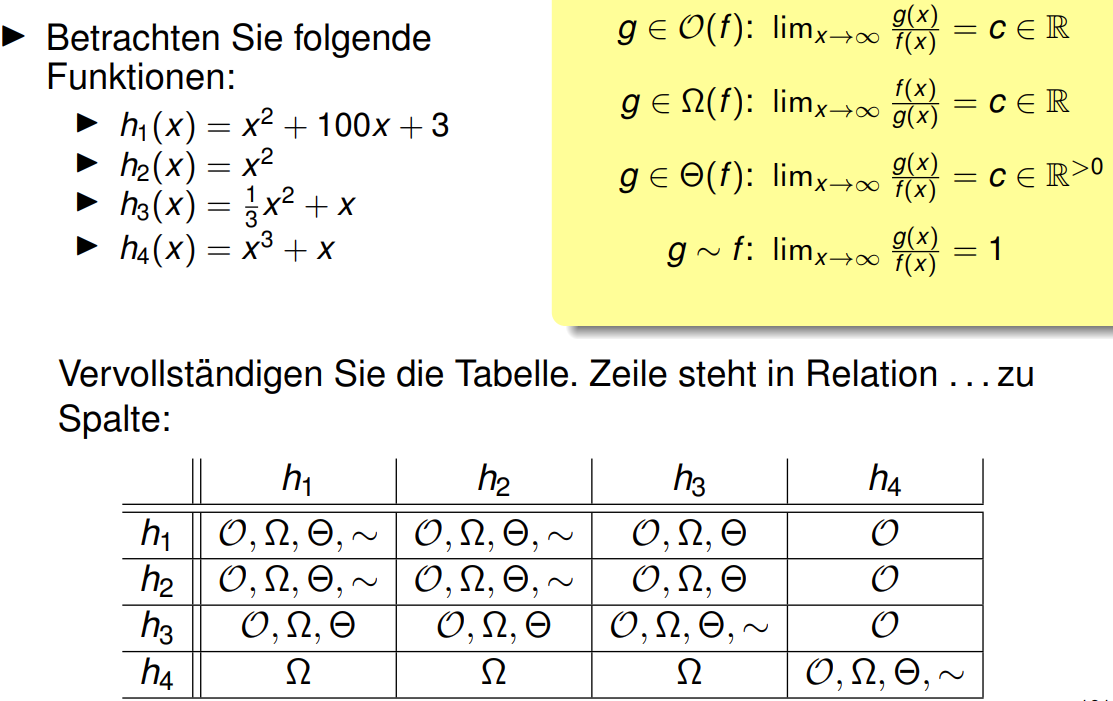
\includegraphics[scale=0.6]{Bilder/landau.PNG}
\end{center}
Zur $\Theta $-Notation gibt es auch ein eigenes \textit{\hyperref[sec:MasterLandau]{Master-Theorem}}.

\subsection{Logarithmen}
Der Logarithmus beschreibt die Umkehrfunktion zur Potenzierung:
\begin{center}
	$\log_a a^b = b$
\end{center}
Wir werden meist den Logarithmus zur Basis 2 brauchen.\newline
Rechenregeln mit dem Logarithmus:
\begin{center}
	$log_ax = \frac{\log_bx}{\log_ba}$\\
	\vspace*{.6cm}
	$\log_ax = \frac{1}{\log_ba}\log_bx = c\log_bx$\\
	\vspace*{.6cm}
	$\mathcal{O}(\log_ax) = \mathcal{O}(c\log_bx) = \mathcal{O}(\log_bx)$ $\Rightarrow $ Die Basis ist für $\mathcal{O}$ irrelevant!
\end{center}

\subsection{Dynamisches Programmieren}
Dynamisches Programmieren ist eine Optimierung der normalen Programmierung. Hierfür werden Probleme in kleinere Teilprobleme aufgeteilt. Die Teilprobleme werden gelöst und dann die Gesamtlösung aus den Teillösungen rekonstruiert.\newline
Die Dynamische Programmierung versagt, wenn...
\vspace{.35cm}
\begin{itemize}
	\item Einzellösungen nicht wiederverwendet werden können
	\item die globale Lösung sich nicht einfach aus lokalen Lösungen zusammensetzen lässt
\end{itemize}
\vspace{.35cm}
Ein Beispiel für die Verwendung der dynamischen Programmierung ist eine rekursive Fibonacci-Funktion.

\subsection{Divide \& Conquer}
Der Divide \& Conquer-Ansatz teilt ein Problem in zwei gleich große Hälften und muss somit nur noch ein halb so großes Problem lösen.\newline
Ein Algorithmus der...
\begin{itemize}
	\item ein Problem in mehrere Teile aufspaltet
	\item die Teilprobleme (rekursiv) löst
	\item die Teillösungen zu einer Gesamtlösung kombiniert
\end{itemize}

\subsection{Greedy Algorithmen}
Greedy-Algorithmen zeichnen sich dadurch aus, dass sie zum aktuellen Zustand $t$ den besten Weg einschlagen und nicht voraus ($t+1$) planen. Anders gesagt: Ein Greedy-Algorithmus entscheidet sich immer für denjenigen Schritt, der ihn dem Ziel am nachsten bringt.

\subsection{Indirektes Sortieren}
Bei sehr großen Datensätzen ist das Sortieren sehr teuer. Um dieses Problem zu umgehen wurde das Indirekte Sortieren erfunden, bei dem nicht die Datensätze getauscht werden, sondern die Indexierung vertauscht wird.

\subsection{Komplexität von rekursiven Algorithmen}
Rekurrenzrelationen? --> Kein Plan? @flo --> HELP

\section{Einfache Sortierverfahren}
\subsubsection{Hase und Igel Algorithmus}
Hierbei gibt es zwei Zeiger auf Elemente in einer einfach verketteten Liste wobei der eine Zeiger beim Iterieren immer ein Element weiter geht und der andere immer 2 weiter. \newline
Hase = 2, Igel = 1
\newpage

\subsection{Selectionsort}
\begin{tabularx}{\textwidth}{l l}
	Speicher: &In-place\\
	Stabilität: &Instabil\\
	Komplexität: &$\mathcal{O}(n^2)$\\
\end{tabularx}
\vspace{.8cm}
\newline
\begin{minipage}[c]{0.7\textwidth}
	\begin{enumerate}
		\item Finde kleinstes Element in Folge($a_0, ...a_{k-1}$)
		\item Vertausche $a_{min}$ mit $a_0$
		\item finde kleinstes Element in Folge($a_1, ...a_{k-1}$)
		\item Vertausche $a_{min}$ mit $a_1$
		\item ...
	\end{enumerate}
\end{minipage}
\begin{minipage}[c]{0.3\textwidth}
	\begin{center}
		\begin{tikzpicture}[scale=0.6]
			\foreach \y in {0,...,4}
			{
				\filldraw[green] (-2.5, 0.5 - \y * 2) rectangle (-2.5 + \y,-0.5 - \y * 2);
				\draw[black,very thick] (-2.5, 0.5 - \y * 2) rectangle (2.5,-0.5 - \y * 2);
				\draw[black,very thick] (-1.5, 0.5 - \y * 2) -- (-1.5,-0.5 - \y * 2);
				\draw[black,very thick] (-0.5, 0.5 - \y * 2) -- (-0.5,-0.5 - \y * 2);
				\draw[black,very thick] (0.5, 0.5 - \y * 2) -- (0.5,-0.5 - \y * 2);
				\draw[black,very thick] (1.5, 0.5 - \y * 2) -- (1.5,-0.5 - \y * 2);
			}
			\node at (-2,0){5};
			\node at (-1,0){8};
			\node at (0,0){3};
			\node at (1,0){9};
			\node at (2,0){1};

			\node at (-2,-2){1};
			\node at (-1,-2){8};
			\node at (0,-2){3};
			\node at (1,-2){9};
			\node at (2,-2){5};
			
			\node at (-2,-4){1};
			\node at (-1,-4){3};
			\node at (0,-4){8};
			\node at (1,-4){9};
			\node at (2,-4){5};
			
			\node at (-2,-6){1};
			\node at (-1,-6){3};
			\node at (0,-6){5};
			\node at (1,-6){9};
			\node at (2,-6){8};
			
			\node at (-2,-8){1};
			\node at (-1,-8){3};
			\node at (0,-8){5};
			\node at (1,-8){8};
			\node at (2,-8){9};

			\draw[red,very thick, <->] (-2,0.5) to[out=60, in=120] (2,0.5);
			\draw[red,very thick, <->] (-1,-1.5) to[out=60, in=120] (0,-1.5);
			\draw[red,very thick, <->] (0,-3.5) to[out=60, in=120] (2,-3.5);
			\draw[red,very thick, <->] (1,-5.5) to[out=60, in=120] (2,-5.5);
		\end{tikzpicture}
	\end{center}
\end{minipage}

\subsection{Insertionsort}
\begin{tabularx}{\textwidth}{l l}
	Speicher: &In-place\\
	Stabilität: &Stabil\\
	Komplexität: &$\mathcal{O}(n^2)$\\
\end{tabularx}
\vspace{.8cm}
\newline
\begin{minipage}[c]{0.7\textwidth}
	\begin{enumerate}
		\item Verwende erstes Element von In als erstes Element von Out
		\item füge zweites Element von In an korrekte Position in Out
		\item füge drittes Element von In an korrekte Position in Out
		\item ...
	\end{enumerate}
\end{minipage}
\begin{minipage}[c]{0.3\textwidth}
	\begin{center}
		\begin{tikzpicture}[scale=0.6]
			\foreach \y in {0,...,4}
			{
				\filldraw[green] (-2.5, 0.5 - \y * 2) rectangle (-1.5 + \y,-0.5 - \y * 2);
				\draw[black,very thick] (-2.5, 0.5 - \y * 2) rectangle (2.5,-0.5 - \y * 2);
				\draw[black,very thick] (-1.5, 0.5 - \y * 2) -- (-1.5,-0.5 - \y * 2);
				\draw[black,very thick] (-0.5, 0.5 - \y * 2) -- (-0.5,-0.5 - \y * 2);
				\draw[black,very thick] (0.5, 0.5 - \y * 2) -- (0.5,-0.5 - \y * 2);
				\draw[black,very thick] (1.5, 0.5 - \y * 2) -- (1.5,-0.5 - \y * 2);
			}
			\node at (-2,0){5};
			\node at (-1,0){8};
			\node at (0,0){3};
			\node at (1,0){9};
			\node at (2,0){1};

			\node at (-2,-2){5};
			\node at (-1,-2){8};
			\node at (0,-2){3};
			\node at (1,-2){9};
			\node at (2,-2){1};
			
			\node at (-2,-4){3};
			\node at (-1,-4){5};
			\node at (0,-4){8};
			\node at (1,-4){9};
			\node at (2,-4){1};
			
			\node at (-2,-6){3};
			\node at (-1,-6){5};
			\node at (0,-6){8};
			\node at (1,-6){9};
			\node at (2,-6){1};
			
			\node at (-2,-8){1};
			\node at (-1,-8){3};
			\node at (0,-8){5};
			\node at (1,-8){8};
			\node at (2,-8){9};

			\draw[red,very thick, ->] (-2,1) -- (-2,0.5);
			\draw[red,very thick, ->] (-1,-0.5) -- (-1,-1.5);
			\draw[red,very thick, ->] (0,-2.5) -- (-2,-3.5);
			\draw[red,very thick, ->] (1,-4.5) -- (1,-5.5);
			\draw[red,very thick, ->] (2,-6.5) -- (-2,-7.5);
		\end{tikzpicture}
	\end{center}
\end{minipage}
\vspace{.6cm}
\newline 
Wen man den Insertionsort In-place verwenden will, sind In und Out gleich.

\subsection{Bubblesort}
\begin{tabularx}{\textwidth}{l l}
	Speicher: &In-place\\
	Stabilität: &Stabil\\
	Komplexität: &$\mathcal{O}(n^2)$\\
\end{tabularx}
\vspace{.8cm}
\newline
\begin{minipage}[c]{0.7\textwidth}
	\begin{enumerate}
		\item durchlaufe eine Folge \textit{S} von Anfang bis Ende
		\begin{enumerate}
			\item wann immer $a_i > a_{i+1}$ gilt, vertausche $a_i$ mit $a_{i+1}$
		\end{enumerate}
		\item wiederhole Schritt 1 solange, bis keine Vertauschungen mehr vorkommen
	\end{enumerate}
\end{minipage}
\begin{minipage}[c]{0.3\textwidth}
	\begin{center}
		\begin{tikzpicture}[scale=0.6]
			\filldraw[green](-2.5,-7.5) rectangle (2.5,-8.5);
			\foreach \y in {0,...,4}
			{
				\draw[black,very thick] (-2.5, 0.5 - \y * 2) rectangle (2.5,-0.5 - \y * 2);
				\draw[black,very thick] (-1.5, 0.5 - \y * 2) -- (-1.5,-0.5 - \y * 2);
				\draw[black,very thick] (-0.5, 0.5 - \y * 2) -- (-0.5,-0.5 - \y * 2);
				\draw[black,very thick] (0.5, 0.5 - \y * 2) -- (0.5,-0.5 - \y * 2);
				\draw[black,very thick] (1.5, 0.5 - \y * 2) -- (1.5,-0.5 - \y * 2);
			}
			\node at (-2,0){5};
			\node at (-1,0){8};
			\node at (0,0){3};
			\node at (1,0){9};
			\node at (2,0){1};

			\draw[red, very thick, <->](-1,0.5) to[out=45, in=135] (0,0.5);
			\draw[red, very thick, <->](1,0.5) to[out=45, in=135] (2,0.5);

			\node at (-2,-2){5};
			\node at (-1,-2){3};
			\node at (0,-2){8};
			\node at (1,-2){1};
			\node at (2,-2){9};
			
			\draw[red, very thick, <->](-2,-1.5) to[out=45, in=135] (-1,-1.5);
			\draw[red, very thick, <->](0,-1.5) to[out=45, in=135] (1,-1.5);
			
			\node at (-2,-4){3};
			\node at (-1,-4){5};
			\node at (0,-4){1};
			\node at (1,-4){8};
			\node at (2,-4){9};
			
			\draw[red, very thick, <->](-1,-3.5) to[out=45, in=135] (0,-3.5);
			
			\node at (-2,-6){3};
			\node at (-1,-6){1};
			\node at (0,-6){5};
			\node at (1,-6){8};
			\node at (2,-6){9};
			
			\draw[red, very thick, <->](-2,-5.5) to[out=45, in=135] (-1,-5.5);
			
			\node at (-2,-8){1};
			\node at (-1,-8){3};
			\node at (0,-8){5};
			\node at (1,-8){8};
			\node at (2,-8){9};
		\end{tikzpicture}
	\end{center}
\end{minipage}

\section{Divide \& Conquer Sortierverfahren}
\subsection{Quicksort}
\begin{tabularx}{\textwidth}{l l}
	Speicher: &In-place\\
	Stabilität: &Instabil\\
	Komplexität: &$\mathcal{O}(n \cdot \log n)$\\
\end{tabularx}
\vspace{.8cm}
\newline
\begin{minipage}[c]{0.6\textwidth}
	\begin{enumerate}
		\item Wenn $|S| \eqslantless 1$: fertig
		\item Wähle Pivot-Element $p \in S$
		\begin{enumerate}
			\item Pivot: Dreh- und Angelpunkt
			\item idealerweise: Mittlere Größe
			\item teile Folge in zwei Teilfolgen S$<$ und S$\geqslant $
			\begin{enumerate}
				\item $\forall_{a \in S<}: a<p$
				\item $\forall_{a \in S\geqslant}: a \geqslant p$
			\end{enumerate}
		\end{enumerate}
		\item Sortiere S$<$ und S$\geqslant $ mittels Quicksort
	\end{enumerate}
\end{minipage}
\begin{minipage}[c]{0.4\textwidth}
	\begin{center}
		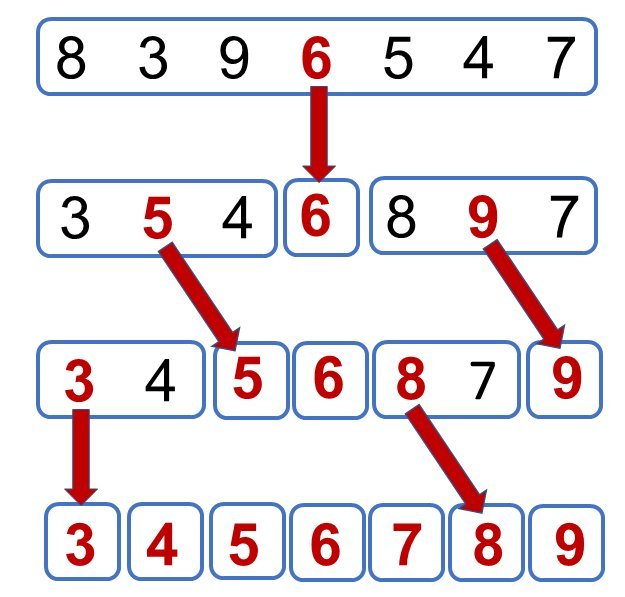
\includegraphics[scale=0.18]{Bilder/quicksort.jpeg}		
	\end{center}
\end{minipage}
\vspace*{0.7cm}
\newline
\textbf{Warum ist Quicksort so effizient?}\newline
Da zuerst grob sortiert und dann immer feiner sortiert wird. Ebenso werden Elemente zwischen denen einmal ein Pivot lag nie wieder miteinander verglichen. \newline
\newline
Neben dem normalen Quicksort gibt es auch den LL-Quicksort-Algorithmus, welcher das Pivot-Element immer mit dem letzten Element der Liste vertauscht und danach alle Elemente kleiner als das Pivot an den Anfang der Liste setzt. Nachdem die ganze Liste durchgelaufen ist, wird das Pivotelement zwischen die kleineren und nicht kleineren Elemente gesetzt. Danach wiederholt sich das Ganze für beide Teillisten.

\subsection{Mergesort(Top-Down)}
\begin{tabularx}{\textwidth}{l l}
	Speicher: &Out-of-place\\
	Stabilität: &Stabil\\
	Komplexität: &$\mathcal{O}(n^2)$\\
\end{tabularx}
\vspace{.8cm}
\newline
\begin{minipage}[c]{0.7\textwidth}
	\begin{enumerate}
		\item Wenn |S| $\leq $ 1: gib S zurück
		\item Teile S in zwei gleich lange Folgen L und R
		\item Sortieren L und R(rekursiv)
		\item Vereinige L und R zu S':
		\begin{enumerate}
			\item solange L oder R nicht leer sind:
			\item m:= min($l_1,r_1$)
			\item entferne m aus L bzw. R
			\item hänge m an S' an
		\end{enumerate}
		\item gib S' zurück
	\end{enumerate}
\end{minipage}
\begin{minipage}[c]{0.3\textwidth}
	\begin{center}
		\begin{tikzpicture}[scale=0.6]
			\draw[black,very thick](-2.5,-0.5) rectangle (2.5,0.5);
			\draw[black, very thick](-1.5,-0.5) -- (-1.5,0.5);
			\draw[red, very thick](-0.5,-0.5) -- (-0.5,0.5);
			\draw[black, very thick](0.5,-0.5) -- (0.5,0.5);
			\draw[black, very thick](1.5,-0.5) -- (1.5,0.5);
			\node at (-2,0){5};
			\node at (-1,0){8};
			\node at (0,0){3};
			\node at (1,0){9};
			\node at (2,0){1};

			\draw[black,very thick](-3,-2.5) rectangle (-1,-1.5);
			\draw[black,very thick](0,-2.5) rectangle (3,-1.5);
			\draw[red, very thick](-2,-2.5) -- (-2,-1.5);
			\draw[red, very thick](2,-2.5) -- (2,-1.5);
			\draw[black, very thick](1,-2.5) -- (1,-1.5);
			\node at (-2.5,-2){5};
			\node at (-1.5,-2){8};
			\node at (0.5,-2){3};
			\node at (1.5,-2){9};
			\node at (2.5,-2){1};

			\draw[black,very thick](-3.25,-3.5) rectangle (-2.25,-4.5);
			\draw[black,very thick](-1.75,-3.5) rectangle (-0.75,-4.5);
			\draw[black,very thick](0,-3.5) rectangle (1,-4.5);
			\draw[black,very thick](1.5,-3.5) rectangle (3.5,-4.5);
			\draw[red, very thick](2.5,-3.5) -- (2.5,-4.5);
			\node at (-2.75,-4){5};
			\node at (-1.25,-4){8};
			\node at (0.5,-4){3};
			\node at (2,-4){9};
			\node at (3,-4){1};

			\draw[black,very thick](1.25,-5.5) rectangle (2.25,-6.5);
			\draw[black,very thick](2.75,-5.5) rectangle (3.75,-6.5);
			\node at (1.75,-6){9};
			\node at (3.25,-6){1};

			\draw[green,very thick](1.5,-7.5) rectangle (3.5,-8.5);
			\draw[green,very thick](2.5,-7.5) -- (2.5,-8.5);
			\node at (2,-8){1};
			\node at (3,-8){9};

			\draw[green,very thick](-3,-9.5) rectangle (-1,-10.5);
			\draw[green,very thick](0,-9.5) rectangle (3,-10.5);
			\draw[green, very thick](-2,-9.5) -- (-2,-10.5);
			\draw[green, very thick](2,-9.5) -- (2,-10.5);
			\draw[green, very thick](1,-9.5) -- (1,-10.5);
			\node at (-2.5,-10){5};
			\node at (-1.5,-10){8};
			\node at (0.5,-10){1};
			\node at (1.5,-10){3};
			\node at (2.5,-10){9};

			\draw[green,very thick](-2.5,-11.5) rectangle (2.5,-12.5);
			\draw[green, very thick](-1.5,-11.5) -- (-1.5,-12.5);
			\draw[green, very thick](-0.5,-11.5) -- (-0.5,-12.5);
			\draw[green, very thick](0.5,-11.5) -- (0.5,-12.5);
			\draw[green, very thick](1.5,-11.5) -- (1.5,-12.5);
			\node at (-2,-12){1};
			\node at (-1,-12){3};
			\node at (0,-12){5};
			\node at (1,-12){8};
			\node at (2,-12){9};

			\draw[->,blue,very thick](5,0) -- (5,-12);
		\end{tikzpicture}
	\end{center}
\end{minipage}

\section{Heap Sortierverfahren}
\subsection{Heapsort}
\begin{tabularx}{\textwidth}{l l}
	Speicher: &In-place\\
	Stabilität: &Instabil\\
	Komplexität: &$\mathcal{O}(n \cdot log(n))$\\
\end{tabularx}
\vspace{.8cm}
\newline
\begin{minipage}[c]{0.5\textwidth}
	\begin{enumerate}
		\item Liste in Baum übertragen
		\item Solange Baum nicht leer:
		\begin{enumerate}
			\item Heapify(Größte nach oben)
			\item Oberste Element in die Liste einfügen
		\end{enumerate}
	\end{enumerate}
\end{minipage}
\begin{minipage}[c]{0.5\textwidth}
	\begin{center}
		\begin{tikzpicture}[scale=0.6]
			\draw[black,very thick](-2.5,-0.5) rectangle (2.5,0.5);
			\draw[black, very thick](-1.5,-0.5) -- (-1.5,0.5);
			\draw[black, very thick](-0.5,-0.5) -- (-0.5,0.5);
			\draw[black, very thick](0.5,-0.5) -- (0.5,0.5);
			\draw[black, very thick](1.5,-0.5) -- (1.5,0.5);
			\node at (-2,0){5};
			\node at (-1,0){8};
			\node at (0,0){3};
			\node at (1,0){9};
			\node at (2,0){1};

			\node[draw, circle] at (0,-2){9};
			\node[draw, circle] at (1.5,-3.5){8};
			\node[draw, circle] at (-1.5,-3.5){3};
			\node[draw, circle] at (3,-5){5};
			\node[draw, circle] at (-3,-5){1};

			\draw[green, very thick, ->](0.75,-2) to[out=45, in=100] (4.5, -3);

			\draw[green,very thick](4,-3) rectangle (9,-4);
			\draw[green, very thick](5,-3) -- (5,-4);
			\draw[green, very thick](6,-3) -- (6,-4);
			\draw[green, very thick](7,-3) -- (7,-4);
			\draw[green, very thick](8,-3) -- (8,-4);
			\node at (4.5,-3.5){9};

			\node[draw, circle] at (0,-6){5};
			\node[draw, circle] at (1.5,-7.5){8};
			\node[draw, circle] at (-1.5,-7.5){3};
			\node[draw, circle] at (-3,-9){1};
			
			\draw[red, very thick, <->](0.75,-6) to[out=0, in=90] (1.5, -6.75);
			\node[text=red] at (6,-7.5){Heapify};

			\node[draw, circle] at (0,-10){8};
			\node[draw, circle] at (1.5,-11.5){5};
			\node[draw, circle] at (-1.5,-11.5){3};
			\node[draw, circle] at (-3,-13){1};

			\draw[green, very thick, ->](0.75,-10) to[out=45, in=100] (5.5, -11);

			\draw[green,very thick](4,-11) rectangle (9,-12);
			\draw[green, very thick](5,-11) -- (5,-12);
			\draw[green, very thick](6,-11) -- (6,-12);
			\draw[green, very thick](7,-11) -- (7,-12);
			\draw[green, very thick](8,-11) -- (8,-12);
			\node at (4.5,-11.5){9};
			\node at (5.5,-11.5){8};

			\node[draw, circle] at (0,-14){5};
			\node[draw, circle] at (-1.5,-15.5){3};
			\node[draw, circle] at (-3,-17){1};

			\node[text=red] at (6,-15.5){Heapify};

			\node at (1.5, -19){...};
		\end{tikzpicture}
	\end{center}
\end{minipage}

\section{Binäre Suchbäume}
\begin{minipage}[c]{0.65\textwidth}
	Ein binärer Suchbaum ist ein Binärbaum mit folgende Eigenschaften:
	\begin{enumerate}
		\item Die Knoten des Baums sind mit Schlüsseln aus einer geordneten Menge \textit{K} beschriftet
		\item Für jeden Knoten gilt:
		\begin{enumerate}
			\item Alle Schlüssel im linken Teilbaum von \textit{N} sind kleiner als der Schlüssel von \textit{N}
			\item Alle Schlüssel im rechten Teilbaum von \textit{N} sind größer als der Schlüssel von \textit{N}
		\end{enumerate}
	\end{enumerate}
\end{minipage}
\begin{minipage}[c]{0.35\textwidth}
	\begin{center}
		\begin{tikzpicture}[scale=.8]
			\draw[->] (0,7) -- (0,6.5);
			\node[draw, circle] (A) at (0,6){8};
			\node[draw, circle] (B) at (-1.5,4){3};
			\node[draw, circle] (C) at (1.5,4){9};
			\node[draw, circle] (D) at (-2.5,2){1};
			\node[draw, circle] (E) at (-0.5,2){5};
			\draw[->] (A) -- (B);
			\draw[->] (A) -- (C);
			\draw[->] (B) -- (D);
			\draw[->] (B) -- (E);
		\end{tikzpicture}
	\end{center}
\end{minipage}

\subsection{Suchen}
\label{sec:SuchenBinaer}
\begin{tabularx}{\textwidth}{l l}
	Komplexität: &$\mathcal{O}(log(n))$\\
\end{tabularx}
\begin{enumerate}
	\item Gegeben: Baum \textit{B} mit Wurzel \textit{W}, Schlüssel \textit{k}
	\item Algorithmus: Suche \textit{k} in \textit{B}
	\begin{enumerate}
		\item Wenn \textit{B} leer ist: Ende, \textit{k} ist nicht in \textit{B}
		\item Wenn \textit{W.key} $>$ \textit{k}: Suche im linken Teilbaum von B
		\item Wenn \textit{W.key} $<$ \textit{k}: Suche im rechten Teilbaum von B
		\item Sonst: \textit{W.key} = \textit{k}; Ende, gefunden
	\end{enumerate}
\end{enumerate}

\subsection{Einfügen}\begin{tabularx}{\textwidth}{l l}
	Komplexität: &$\mathcal{O}(log(n))$\\
\end{tabularx}
\begin{enumerate}
	\item Gegeben: Baum \textit{B} mit Wurzel \textit{W}, Schlüssel \textit{k}
	\item Gesucht: Baum \textit{B'}, der aus \textit{B} entsteht, wenn \textit{k} eingefügt wird
	\item Idee:
	\begin{enumerate}
		\item Suche nach \textit{k}
		\item Falls \textit{k} nicht in \textit{B} ist, setze es an der Stelle ein, an der es gefunden worden wäre
	\end{enumerate}
	\item Implementierung z.B. funktional:
	\begin{enumerate}
		\item Wenn \textit{B} leer ist, dann ist ein Baum mit einem Knoten mit Schlüssel \textit{k} der gesuchte Baum
		\item Ansonsten:
		\begin{enumerate}
			\item Wenn \textit{W.key} $>$ \textit{k}: Ersetze den linken Teilbaum von \textit{B} durch den Baum, der entsteht, wenn man \textit{k} in ihn einfügt
			\item Wenn \textit{W.key} $<$ \textit{k}: Ersetze den rechten Teilbaum von \textit{B} durch den Baum, der entsteht, wenn man \textit{k} in ihn einfügt
			\item Ansonsten: \textit{k} ist schon im Baum
		\end{enumerate}
	\end{enumerate}
\end{enumerate}

\subsection{Löschen}
Beim Löschen in Binärbäumen muss man beachten, dass der zu löschende Knoten auch Nachfolger haben kann. Aus diesem Grund gibt es hierbei eine Fallunterscheidung:\newline \newline
\begin{tabularx}{\textwidth}{l l}
	Komplexität: &$\mathcal{O}(log(n))$\\
\end{tabularx}
\begin{enumerate}
	\item Problem: Entferne einen Knoten \textit{K} mit gegebenen Schlüssel \textit{k} aus dem Suchbaum
	\begin{enumerate}
		\item ... und erhalte die Binärbaumeigenschaft
		\item ... und erhalte die Suchbaumeigenschaft
	\end{enumerate}
	\item Fallunterscheidung:
	\begin{enumerate}
		\item Fall 1: Knoten hat \textcolor{blue}{keinen} Nachfolger
		\begin{enumerate}
			\item Lösung: Schneide Knoten ab
			\item Korrektheit: Offensichtlich
		\end{enumerate}
		\item Fall 2: Knoten hat \textcolor{blue}{einen} Nachfolger
		\begin{enumerate}
			\item Lösung: Ersetze Knoten durch seinen einzigen Nachfolger
			\item Korrektheit: Alle Knoten in diesem Baum sind größer(bzw. kleiner) als die Knoten im Vorgänger des gelöschten Knotens
		\end{enumerate}
		\item Fall 3: Knoten hat \textcolor{blue}{zwei} Nachfolger
		\begin{enumerate}
			\item Lösung: 
			\begin{enumerate}
				\item Suche größten Knoten \textit{G} im linken Teilbaum
				\item Tausche \textit{G} und \textit{K} (oder einfacher: Ihre Schlüssel/Werte)
				\item Lösche rekursiv \textit{k} im linken Teilbaum von (nun) \textit{G}
			\end{enumerate}
		\end{enumerate}
	\end{enumerate}
\end{enumerate}

\subsection{Ausgabe}
\label{sec:AusgabeBinaer}
\begin{tabularx}{\textwidth}{l l}
	Komplexität: &$\mathcal{O}(n)$\\
\end{tabularx}
\begin{enumerate}
	\item Gegeben: Baum \textit{B} mit Wurzel \textit{W}
	\item Algorithmus: Gib alle \textit{W} in \textit{B} aus
	\begin{enumerate}
		\item Wenn \textit{B} leer ist: Ende
		\item Ausgabe(\textit{W}) ist rekursiv:
		\begin{enumerate}
			\item Wenn \textit{W.linkes Kind} existiert: Ausgabe(\textit{W.linker Teilbaum})
			\item Gib \textit{W} aus
			\item Wenn \textit{W.rechtes Kind} existiert: Ausgabe(\textit{W.rechter Teilbaum})
		\end{enumerate}
	\end{enumerate}
\end{enumerate}

\subsection{Balacierte und Unbalancierte Bäume}
\begin{minipage}[c]{0.6\textwidth}
	Binärbaume können entarten, indem man zum Beispiel eine sortierte Liste in einen Binärbaum umwandelt. In diesem Fall entsteht solch ein unbalacierter Baum:\vspace{2cm}\newline
	Diese entarteten Binärbäume sind sehr ineffizient und sollten rebalanciert werden. Die Rebalancierung zu Balancierten Binärbäumen geschieht zum Beispiel bei AVL-Bäumen.
\end{minipage}
\begin{minipage}[c]{0.4\textwidth}
	\begin{center}
		\begin{tikzpicture}[scale=.8]
			\draw[->] (0.5,7) -- (0.5,6.5);
			\node[draw, circle] (A) at (0.5,6){1};
			\node[draw, circle] (B) at (1.5,4){3};
			\node[draw, circle] (C) at (2.5,2){5};
			\node[draw, circle] (D) at (3.5,0){8};
			\node[draw, circle] (E) at (4.5,-2){9};
			\draw[->] (A) -- (B);
			\draw[->] (B) -- (C);
			\draw[->] (C) -- (D);
			\draw[->] (D) -- (E);
		\end{tikzpicture}
	\end{center}
\end{minipage}

\section{AVL-Bäume}
	Binäre Suchbäume mit maximaler Höhendifferenz von 2.\\
	\textbf{Begriffe:}\\
	\begin{enumerate}
		\item Höhe/Tiefe: Anzahl der Knoten auf dem längsten Ast
		\item Gewicht: Anzahl der Knoten
		\item Balance: Tiefenunterschied ist nicht Höher als 2
	\end{enumerate}

\subsection{Rotieren}
Beim Rotieren gibt es zwei unterschiedliche Arten zu rotieren. Hierbei wird unterschieden zwischen Rechts-Rotation und Links-Rotation.\newline
\textbf{Rechts-Rotation:}\newline
\begin{center}
	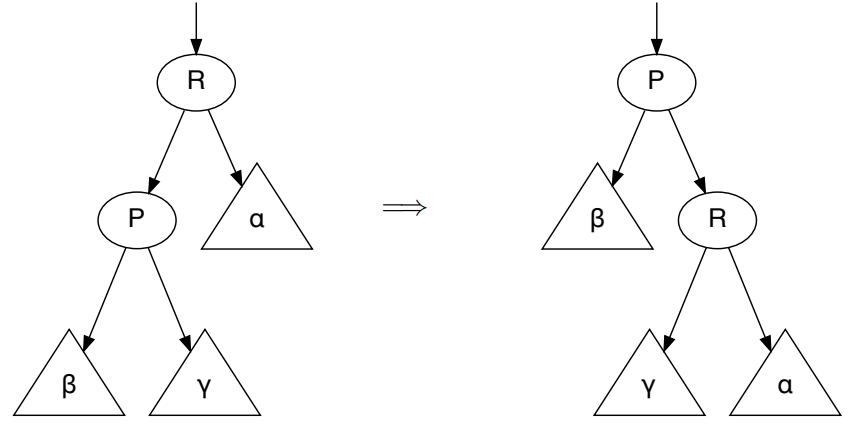
\includegraphics[scale=1]{Bilder/AVL_rechts_rot.PNG}
\end{center}
\textbf{Links-Rotation:}\newline
\begin{center}
	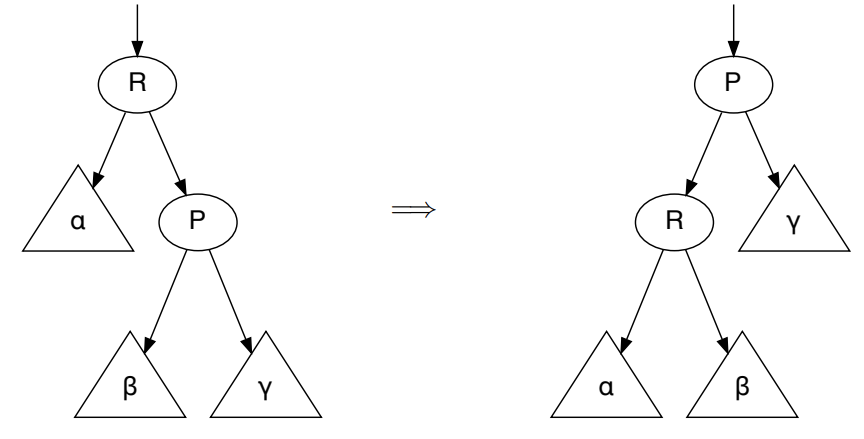
\includegraphics[scale=1]{Bilder/AVL_links_rot.PNG}
\end{center}

\subsection{Balancieren}
Wenn ein Baum keine AVL-Bedingungen erfüllt, da die Balance der Teilbäume eine Differenz $\geq $2 hat, muss er rebalanciert werden. Diese Rebalancierung geschieht durch Rechts- oder Links-Rotationen. Jeder Baum kann als AVL-Baum dargestellt werden!

\subsection{Suchen}
Gleich wie das \textit{\hyperref[sec:SuchenBinaer]{Suchen}} beim Binärbaum.

\subsection{Ausgabe}
Gleich wie die \textit{\hyperref[sec:AusgabeBinaer]{Ausgabe}} beim Binärbaum.

\subsection{Einfügen}
\begin{tabularx}{\textwidth}{l l}
	Komplexität: &$\mathcal{O}(\log n)$\\
\end{tabularx}
\begin{enumerate}
	\item füge Knoten wie in gewöhnlichen Binärbaum ein
	\item durchlaufe Baum vom neuen Knoten bis zur Wurzel, passe Balance Anders
	\item wenn im Knoten \textit{k} der Höhenunterschied 2 (oder -2) ist: führe Links- (oder Rechts-) Rotation durch
	\begin{enumerate}
		\item wenn das Pivot \textit{p} ein \textcolor{blue}{anderes} Vorzeichen hat als die Wurzel: \textcolor{blue}{Doppelrotation}
		\begin{enumerate}
			\item \textcolor{blue}{Rechts-} Rotation mit \textit{p} als Wurzel
			\item \textcolor{blue}{Links-} Rotation mit \textit{k} als Wurzel
		\end{enumerate}
		\item sonst (gleiches Vorzeichen): Einzelrotation
		\begin{enumerate}
			\item \textcolor{blue}{Links-} Rotation mit \textit{k} als Wurzel
		\end{enumerate}
	\end{enumerate}
\end{enumerate}
Balanceanpassungen gibt es nur auf dem aktuellen Pfad(bottom-up) und es ist maximal eine Doppelrotation notwendig!

\subsection{Löschen}
\begin{tabularx}{\textwidth}{l l}
	Komplexität: &$\mathcal{O}(\log n)$\\
\end{tabularx}
\begin{enumerate}
	\item lösche Knoten wie aus gewöhnlichem Binärbaum
	\item durchlaufe Baum vom gelöschten Knoten zur Wurzel
	\item wenn der Hohenunterschied 2 (oder -2) ist: führe Links- (oder Rechts-) Rotation durch
	\begin{enumerate}
		\item wenn das Pivot ein \textcolor{blue}{anderes} Vorzeichen hat als die Wurzel: \textcolor{blue}{Doppelrotation}
		\item sonst (gleiches Vorzeichen oder 0): Einzelrotation
	\end{enumerate}
\end{enumerate}
Hierbei sind möglicherweise \textcolor{blue}{mehrere} Rotationen notwendig!

\section{Hashing und Hashtabellen}
Hashtabellen haben die besondere Eigenschaft, dass alle Funktionen außer das Ausgaben eine Komplexität von $\mathcal{O}(1)$ haben. Hierbei werden die Datensätze in einer endlichen Tabelle gespeichert. Die Speicherung erfolgt nach einem speziellen Verfahren namens Hashing. Hierfür wird eine Hashfunktion geschrieben, welche folgende Eigenschaften erfüllen muss:
\begin{enumerate}
	\item Berücksichtigung aller Bits
	\begin{enumerate}
		\item Änderung von \textit{i} um 1 Bit $\rightsquigarrow$ Änderung von \textit{h(i)}
		\item Vermeidung von gleichen Hash-Werten(\textcolor{blue}{Kollisionen})
		\item Schlecht: Gleicher Hash-Wert für Schmidt, Schmid und Schmied
	\end{enumerate}
	\item kleine Änderungen von \textit{i} $\rightsquigarrow$ große Änderung von \textit{h(i)}
	\begin{enumerate}
		\item Gleichmäßige Verteilung ähnlicher Schlüssel
		\item Schlecht: Alle Schmidts liegen dicht beieinander
		\item Vermeidung von \textcolor{blue}{Clustering}
	\end{enumerate}
\end{enumerate}
\textbf{\textcolor{blue}{Kollision}}\newline
Eine Kollision tritt auf, wenn zwei verschiedene Schlüssel, die denselben Hash-Wert haben, in eine Hash-Tabelle eingefügt werden.\newline
\newline
\textbf{\textcolor{blue}{Clustering}}\newline
Wenn in einer Hashtabelle mehrere Schlüssel in Zellen nebeneinander liegen und somit einen Häufungspunkt in der Tabelle bilden.\newline
\newline
Um die Kollisionen zu behandeln gibt es zwei Möglochkeiten:

\subsection{Linear Probing}
Beim Linear Probing wird der aktuelle Schlüssel bei einer Kollision einfach in die nächste freie Zelle geschrieben (Also beim Hashwert + 1). Am Ende der Liste wird wieder zum Anfang gesprungen.\newline
Hierbei gibt es den Nachteil dass sich sehr schnell Cluster bilden und somit die Hashtabelle ineffizient wird.

\subsection{Re-Hashing}
Beim Re-Hashing gibt es eine zweite Hash-Funktion welche bei Kollisionen zum Einsatz kommt. Diese bestimmt die Sprungweite. Am Besten ist es, wenn die Sprungweite eine Primzahl ist und somit kein Teiler der Tabellengröße sein kann. Mit dieser Methode kann das Problem der Clusterbildung umgangen werden.

\section{Graph-Algorithmen}
Ein Graph ist entweder gerichtet oder ungerichtet. Gerichtete Graphen haben eine Richtung wobei ungerichtete Graphen beidseitig anwendbar sind(symmetrisch sind). Ebenso können Graphen gewichtet sein in dem sie beschriftet sind. Hierbei besteht eine Gewichtung wenn ein Graph mit einer Zahl versehen ist.

\subsection{Adjazenzmatrix}
Die Adjazenzmatrix kann als zweidimensionales Array betrachtet werden. Hierbei wird die Verbindung aller Punkte miteinander aufgelistet:\newline
\newline
\begin{minipage}[c]{0.7\textwidth}
	\begin{center}
		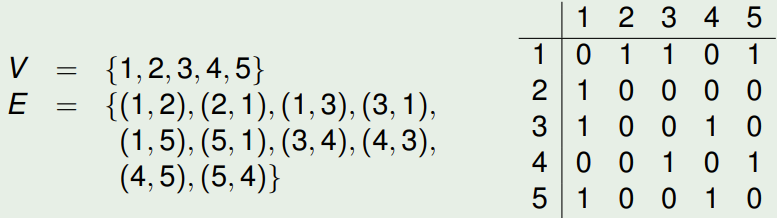
\includegraphics[scale=.8]{Bilder/Adjazenzmatrix.PNG}
	\end{center}
\end{minipage}
\begin{minipage}[c]{0.3\textwidth}
	\begin{center}
		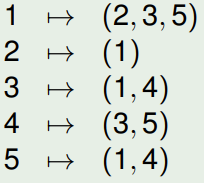
\includegraphics[scale=.95]{Bilder/Adjazenzliste.PNG}
	\end{center}
\end{minipage}\vspace{.5cm}
\textit{V} beschreibt die Punkte die miteinander verbunden sind und \textit{E} ist eine Menge aller bestehenden Graphen zwischen diesen Punkten. Rechts befindet sich die zugehörige Adjazenzliste \textit{L}.\newline
Die Adjazenzliste ist gegenüber der Matrix in nicht so dichten Graphen deutlich platzsparender und wird vorallem bei mageren Graphen eingesetzt. Jedoch ist die Komplexität bei der Adjazenzliste höher als bei der Matrix($\mathcal{O}(N)$ statt $\mathcal{O}(1)$)

\subsection{Pfad, Zyklus und Baum}
Ein \textcolor{blue}{Pfad} ist eine Folge von Knoten.\newline
Ein \textcolor{blue}{Zyklus} ist nichtleerer Pfad. \newline
Ein \textcolor{blue}{Baum} ist ein verbundener azyklischer Baum.

\subsection{Minimale Spannbäume \& Algorithmus von Prim}
Minimale Spannbäume sind Netze, welche möglichst effizient und minimalistisch vernetzt sind. Hierbei sollen aber trotzdem alle Knoten von allen anderen Knoten erreichbar sein. \textbf{Tipp:} Minimale Spannbäume mit \textit{n} Knoten haben \textit{n - 1} Kanten! \newline
Kürzeste Pfade beschreiben den kürzesten Weg(bzgl. Gewichtung) zwischen zwei Knoten.\newline
\newline
Der Algortihmus von Prim ist ein Greedy-Algorithmus und findet immer den minimalen Spannbaum in einem Graph. Hierbei ist egal wo man beginnt, das Ergebnis ist immer das Gleiche.\newline
Eingabe: Graph $G = (V, E)$\newline
Ausgabe: MST $T = (V, E_T)$
\begin{enumerate}
	\item $E_T=0$
	\item Wähle $V_{start}; V_b = {V_{start}}; V_n = V \backslash {V_{start}}$
	\item solange $V_n$ Knoten enthält
	\begin{enumerate}
		\item $e_n = (v_b, v_n)$ sei billigste Kante zwischen Knoten aus $V_b$ und $V_n$
		\item nimm $e_n$ zu $E_T$ hinzu
		\item entferne $v_n$ aus $V_n$
		\item nimm $v_n$ zu $V_b$ hinzu 
	\end{enumerate}
	\item gib $(V, E_T)$ zurück
\end{enumerate}
\begin{tabularx}{\textwidth}{l l}
	Komplexität: &$\mathcal{O}(|V|^3)$\\
\end{tabularx}
Kann aber durch Optimierungen auf $\mathcal{O}(|V|^2 \cdot \log |V|)$ gebracht werden.

\subsection{Kürzeste Wege/Dijkstra}
Dijkstra's Algortihmus ist ebenfalls ein Greedy-Algorithmus. \newline
Eingabe: Graph $(V, E)$, Kantengewichtsfunktion $e$, Startknoten $v_s$\newline
Ausgabe: Funktion $d : V \longmapsto \mathbb{N} $ mit Entfernung von $v_s$\newline
Variablen: Liste der besuchten Knoten $B$, aktueller Knoten $v_c$
\begin{enumerate}
	\item Setze $d(v_s) = 0, d(v_i) = \infty$ für alle $v_i \neq v_s, B = 0$
	\item Setze $v_c = v_s$
	\item Für alle Nachbarn $v$ von $v_c$:
	\begin{enumerate}
		\item Berechne $d_{tmp} = d(v_c) + e(v_c, v)$
		\item Wenn $d_{tmp} < d(v)$ gilt, setze $d(v) = d_{tmp}$
	\end{enumerate}
	\item Füge $v_c$ zu $B$ hinzu
	\item Wenn $B = V$ gilt: fertig (oder wenn für alle Knoten $v \in V \backslash B$ gilt: $d(v) = \infty$)
	\item Sonst: Wähle als neuen $v_c$ den Knoten aus $V \backslash B$ mit geringster Entfernung
	\item Fahre bei 3 fort
\end{enumerate}
\begin{tabularx}{\textwidth}{l l}
	Komplexität: &$\mathcal{O}(|V|^2)$\\
\end{tabularx}

\section{Master-Theorem}
Bedingungen für das Verwenden des Master-Theorems:
\begin{enumerate}
	\item Mindestens eine Teilung durch 2
	\item Rekurrenz vorhanden \textcolor{red}{??}
\end{enumerate}
\begin{center}
	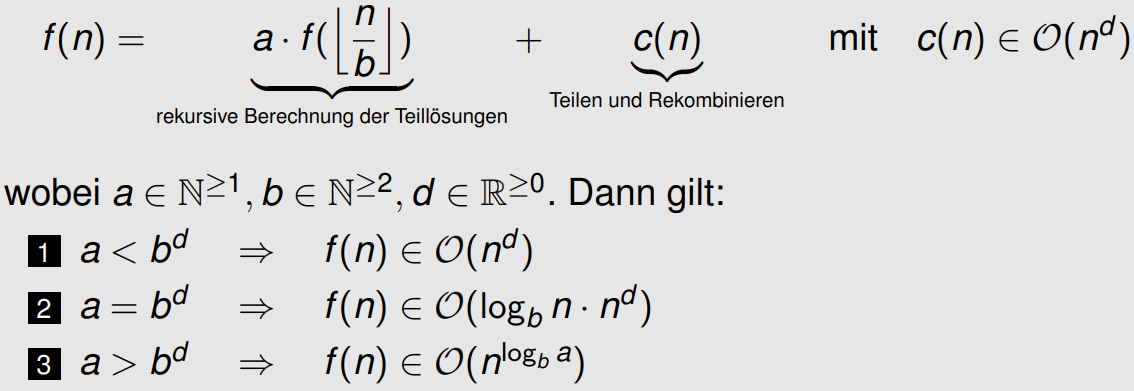
\includegraphics[scale=.8]{Bilder/MasterTheorem.PNG}
\end{center}
\textbf{Beispiele:}\newline
\textit{Wenden Sie das Master Theorem auf folgende Rekurrenzgleichung an:} $f(n)= 4\cdot f(\frac{n}{2}) +  n$\newline
\begin{center}
	$a = 4; b = 2$ $\rightsquigarrow $ Fall 3: $a>b^d$; d = 1;\newline
	$f(n) \in \mathcal{O}(n^{\log_2 4}) = \mathcal{O}(n^2)$
\end{center}
\vspace{.8cm}
\textit{Wenden Sie das Master Theorem auf folgende Rekurrenzgleichung an:} $f(n)= 4\cdot f(\frac{n}{2}) +  n^2$\newline
\begin{center}
	$a = 4; b^d = 2^2 = 4$ $\rightsquigarrow $ Fall 2: $a=b^d$; d = 2;\newline
	$f(n) \in \mathcal{O}(\log_2 n \cdot n^2)$
\end{center}

\section{Master-Theorem nach Landau}
\label{sec:MasterLandau}
Hierbei wird das Master Theorem zur Berechnung von $\Theta $ verwendet:\newline
\begin{center}
	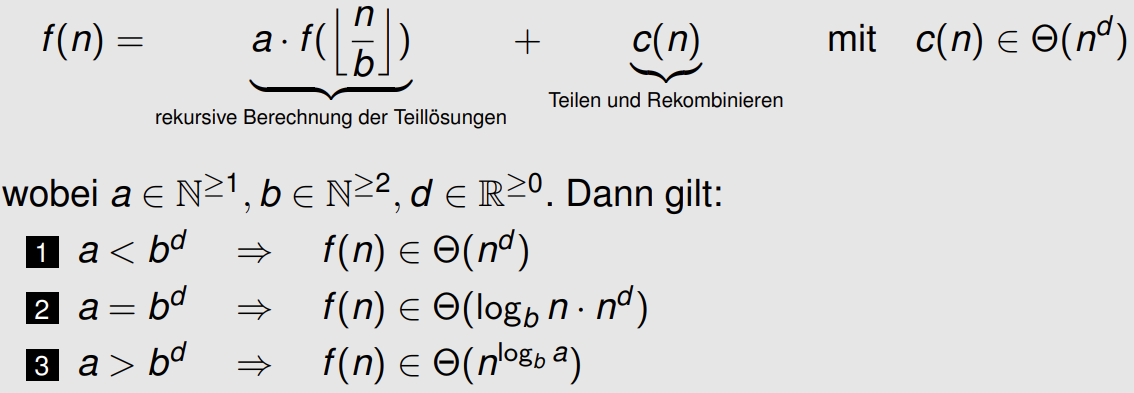
\includegraphics[scale=.8]{Bilder/MasterTheoremLandau.PNG}
\end{center}

\end{document}